\documentclass{article}
%%%%%%%%%%%%%%%%%%%%%%%%%%%%%%%%%%%%%%%%%
% Lachaise Assignment
% Structure Specification File
% Version 1.0 (26/6/2018)
%
% This template originates from:
% http://www.LaTeXTemplates.com
%
% Authors:
% Marion Lachaise & François Févotte
% Vel (vel@LaTeXTemplates.com)
%
% License:
% CC BY-NC-SA 3.0 (http://creativecommons.org/licenses/by-nc-sa/3.0/)
% 
%%%%%%%%%%%%%%%%%%%%%%%%%%%%%%%%%%%%%%%%%

%----------------------------------------------------------------------------------------
%	PACKAGES AND OTHER DOCUMENT CONFIGURATIONS
%----------------------------------------------------------------------------------------

\usepackage{amsmath,amsfonts,stmaryrd,amssymb,subcaption} % Math packages

\usepackage{enumerate} % Custom item numbers for enumerations

\usepackage[ruled]{algorithm2e} % Algorithms

\usepackage[framemethod=tikz]{mdframed} % Allows defining custom boxed/framed environments

\usepackage{listings} % File listings, with syntax highlighting
\lstset{
	basicstyle=\ttfamily, % Typeset listings in monospace font
}

%----------------------------------------------------------------------------------------
%	DOCUMENT MARGINS
%----------------------------------------------------------------------------------------

\usepackage{geometry} % Required for adjusting page dimensions and margins

\geometry{
	paper=a4paper, % Paper size, change to letterpaper for US letter size
	top=2cm, % Top margin
	bottom=2.5cm, % Bottom margin
	left=2cm, % Left margin
	right=2cm, % Right margin
	headheight=14pt, % Header height
	footskip=1.5cm, % Space from the bottom margin to the baseline of the footer
	headsep=1.2cm, % Space from the top margin to the baseline of the header
	%showframe, % Uncomment to show how the type block is set on the page
}

%----------------------------------------------------------------------------------------
%	FONTS
%----------------------------------------------------------------------------------------

\usepackage[utf8]{inputenc} % Required for inputting international characters
\usepackage[T1]{fontenc} % Output font encoding for international characters

\usepackage{XCharter} % Use the XCharter fonts

%----------------------------------------------------------------------------------------
%	COMMAND LINE ENVIRONMENT
%----------------------------------------------------------------------------------------

% Usage:
% \begin{commandline}
%	\begin{verbatim}
%		$ ls
%		
%		Applications	Desktop	...
%	\end{verbatim}
% \end{commandline}

\mdfdefinestyle{commandline}{
	leftmargin=10pt,
	rightmargin=10pt,
	innerleftmargin=15pt,
	middlelinecolor=black!50!white,
	middlelinewidth=2pt,
	frametitlerule=false,
	backgroundcolor=black!5!white,
	frametitle={Command Line},
	frametitlefont={\normalfont\sffamily\color{white}\hspace{-1em}},
	frametitlebackgroundcolor=black!50!white,
	nobreak,
}

% Define a custom environment for command-line snapshots
\newenvironment{commandline}{
	\medskip
	\begin{mdframed}[style=commandline]
}{
	\end{mdframed}
	\medskip
}

%----------------------------------------------------------------------------------------
%	FILE CONTENTS ENVIRONMENT
%----------------------------------------------------------------------------------------

% Usage:
% \begin{file}[optional filename, defaults to "File"]
%	File contents, for example, with a listings environment
% \end{file}

\mdfdefinestyle{file}{
	innertopmargin=1.6\baselineskip,
	innerbottommargin=0.8\baselineskip,
	topline=false, bottomline=false,
	leftline=false, rightline=false,
	leftmargin=2cm,
	rightmargin=2cm,
	singleextra={%
		\draw[fill=black!10!white](P)++(0,-1.2em)rectangle(P-|O);
		\node[anchor=north west]
		at(P-|O){\ttfamily\mdfilename};
		%
		\def\l{3em}
		\draw(O-|P)++(-\l,0)--++(\l,\l)--(P)--(P-|O)--(O)--cycle;
		\draw(O-|P)++(-\l,0)--++(0,\l)--++(\l,0);
	},
	nobreak,
}

% Define a custom environment for file contents
\newenvironment{file}[1][File]{ % Set the default filename to "File"
	\medskip
	\newcommand{\mdfilename}{#1}
	\begin{mdframed}[style=file]
}{
	\end{mdframed}
	\medskip
}

%----------------------------------------------------------------------------------------
%	NUMBERED QUESTIONS ENVIRONMENT
%----------------------------------------------------------------------------------------

% Usage:
% \begin{question}[optional title]
%	Question contents
% \end{question}

\mdfdefinestyle{question}{
	innertopmargin=1.2\baselineskip,
	innerbottommargin=0.8\baselineskip,
	roundcorner=5pt,
	nobreak,
	singleextra={%
		\draw(P-|O)node[xshift=1em,anchor=west,fill=white,draw,rounded corners=5pt]{%
		Question \theQuestion\questionTitle};
	},
}

\newcounter{Question} % Stores the current question number that gets iterated with each new question

% Define a custom environment for numbered questions
\newenvironment{question}[1][\unskip]{
	\bigskip
	\stepcounter{Question}
	\newcommand{\questionTitle}{~#1}
	\begin{mdframed}[style=question]
}{
	\end{mdframed}
	\medskip
}

%----------------------------------------------------------------------------------------
%	WARNING TEXT ENVIRONMENT
%----------------------------------------------------------------------------------------

% Usage:
% \begin{warn}[optional title, defaults to "Warning:"]
%	Contents
% \end{warn}

\mdfdefinestyle{warning}{
	topline=false, bottomline=false,
	leftline=false, rightline=false,
	nobreak,
	singleextra={%
		\draw(P-|O)++(-0.5em,0)node(tmp1){};
		\draw(P-|O)++(0.5em,0)node(tmp2){};
		\fill[black,rotate around={45:(P-|O)}](tmp1)rectangle(tmp2);
		\node at(P-|O){\color{white}\scriptsize\bf !};
		\draw[very thick](P-|O)++(0,-1em)--(O);%--(O-|P);
	}
}

% Define a custom environment for warning text
\newenvironment{warn}[1][Warning:]{ % Set the default warning to "Warning:"
	\medskip
	\begin{mdframed}[style=warning]
		\noindent{\textbf{#1}}
}{
	\end{mdframed}
}

%----------------------------------------------------------------------------------------
%	INFORMATION ENVIRONMENT
%----------------------------------------------------------------------------------------

% Usage:
% \begin{info}[optional title, defaults to "Info:"]
% 	contents
% 	\end{info}

\mdfdefinestyle{info}{%
	topline=false, bottomline=false,
	leftline=false, rightline=false,
	nobreak,
	singleextra={%
		\fill[black](P-|O)circle[radius=0.4em];
		\node at(P-|O){\color{white}\scriptsize\bf i};
		\draw[very thick](P-|O)++(0,-0.8em)--(O);%--(O-|P);
	}
}

% Define a custom environment for information
\newenvironment{info}[1][Info:]{ % Set the default title to "Info:"
	\medskip
	\begin{mdframed}[style=info]
		\noindent{\textbf{#1}}
}{
	\end{mdframed}
}
 % Include the file specifying the document structure and custom commands
\setlength\parindent{0pt}

\title{EECS 545: Homework \#1} % Title of the assignment

\author{Mingliang Duanmu\\ \texttt{duanmuml@umich.edu}} % Author name and email address

\date{\today} % University, school and/or department name(s) and a date

\begin{document}

\maketitle % Print the title

\section{Linear regression on a polynomial}

\subsection*{a}
\subsubsection*{i}
For both methods, we have iterations = 1000, learning rate = 0.01, and degree = 2. \\
For batch gradient descent, we have coefficients = array([-2.82412688,  1.94687097]). \\
For stochastic gradient descent, we have coefficients = array([-2.82979555,  1.942896  ]).

\subsubsection*{ii}
We use the same parameters as before, iterations = 1000, learning rate = 0.01, and degree = 2. \\
Since the training data is relatively small, we do not notice a distinct difference in speed of convergence, but by printing out the $E_{MS}$ for the first 100 epochs, we find batch gradient descent converges a little faster than stochastic gradient descent.

\subsection*{b}
\subsubsection*{i}
\begin{figure}[htbp]
    \centering
    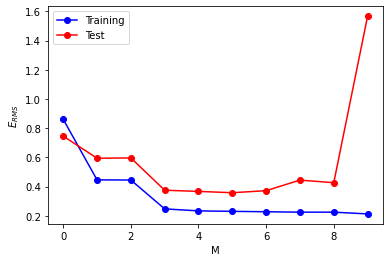
\includegraphics[width=0.5\textwidth]{1bi.png}
\end{figure}

\subsubsection*{ii}
From the plot we find the polynomial with $M = 5$ best fits the data since the RMS error of the test data is minimized. If the degree is high ($M = 9$), we can see the testing error is much greater than training error, which is an over-fitting. When the degree is too small ($M < 3$), we can see both training and testing error are great, which is an under-fitting.

\newpage

\subsection*{c}
\subsubsection*{i}
The closed form solution for ridge regression is
$$\mathbf{w} = (\mathbf{\Phi}^T\mathbf{\Phi} + \lambda\mathbf{I})^{-1}\mathbf{\Phi}^T\mathbf{Y}$$

\begin{figure}[htbp]
    \centering
    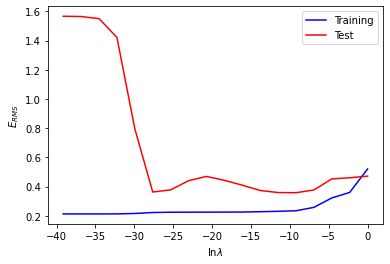
\includegraphics[width=0.5\textwidth]{1ci.png}
\end{figure}

\subsubsection*{ii}
From the plot above we observe that when $\lambda = 10^{-4}$ the test error is minimized.

\newpage

\section{Locally weighted linear regression}

\subsection*{a}
$$E_D(\mathbf{w}) = (X\mathbf{w} - \mathbf{y})^TR(X\mathbf{w} - \mathbf{y}) = \mathbf{z}^T R \mathbf{z} = \sum_{i=1}^{N} R^{(i)}z_i^2 = \frac{1}{2}\sum_{i=1}^{N} r^{(i)}(z_i)^2$$
where $z_i = \mathbf{w}^Tx^{(i)-y^{(i)}}$. So we have
$$R = \frac{1}{2} diag(r_1, r_2, \cdots, r_N)$$

\subsection*{b}
$$E_D(\mathbf{w}) = \frac{1}{2} \sum_{i=1}^{N} r^{(i)}(\mathbf{w}^T x^{(i)})^2 - \sum_{i=1}^{N}r^{(i)}y^{(i)} \mathbf{w}^T (x^{(i)})^2 + \frac{1}{2} \sum_{i=1}^{N} r^{(i)}(y^{(i)})^2$$
$$= \frac{1}{2}\mathbf{w}^TX^T \mathbf{R} X\mathbf{w} - \mathbf{w}^TX^T \mathbf{R}Y + \frac{1}{2}Y^T\mathbf{R}Y$$
By calculating the gradient of expectation and set to zero,
$$\nabla E_D(\mathbf{w}) = X^T \mathbf{R}X\mathbf{w} - X^T\mathbf{R}Y = 0$$
So we have the close form
$$\mathbf{w} = (X^T\mathbf{R}X)^{-1}X^T\mathbf{R}X$$
\subsection*{c}
$$\log P(Y|X, \mathbf{w}) = \log P(y^{(1)}, y^{(2)}, \cdots, y^{(N)}|X, \mathbf{w})$$
$$= \sum_{i=1}^{N} \log [\frac{1}{\sqrt{2 \pi} \sigma} \exp (-\frac{\|y^{(i)}-W^{T} x^{(i)}\|^{2}}{2(\sigma^{(i)})^{2}})]$$
$$= \sum_{i=1}^{N} (-\frac{1}{2}\log(2\pi) - \log(\sigma^{(i)}) - \frac{\|y^{(i)}-W^{T} x^{(i)}\|^{2}}{2(\sigma^{(i)})^{2}})$$
$$= -\frac{N}{2}\log(2\pi) - \sum_{i=1}^{N} \log(\sigma^{(i)} - \sum_{i=1}^{N} \frac{\|y^{(i)}-W^{T} x^{(i)}\|^{2}}{2(\sigma^{(i)})^{2}})$$
Let $\beta^{(i)} = \frac{1}{\sigma^{(i)}}$ and calculate the gradient and set to zero,
$$\nabla \log P(Y|X, \mathbf{w}) = \sum_{i=1}^{N} X(y^{(i)} - \mathbf{w}^T)x^{(i)}x^{(n)}\beta^{(i)}$$
$$= \sum_{i=1}^{N} y^{(i)}x^{(i)}\beta^{(i)} - x^{(i)}(x^{(i)})^T \mathbf{w} \beta^{(i)} = X^T\beta Y - X^T\beta X\mathbf{w} = 0$$
The maximum likelihood estimate of $\mathbf{w}$ can be written as $(X^T\beta X)^{-1}X^T\beta Y$, where $\beta = diag(\frac{1}{\sigma^{(1)}}, \frac{1}{\sigma^{(1)}}, \cdots, \frac{1}{\sigma^{(N)}})$ is a diagonal matrix like $\mathbf{R}$ in the previous question. Therefore, finding the maximum likelihood estimate of $\mathbf{w}$ reduces to solving a weighted linear regression problem.

\newpage

\subsection*{d}
\subsubsection*{i}
\begin{figure}[htbp]
    \centering
    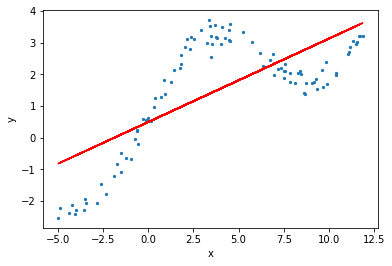
\includegraphics[width=0.5\textwidth]{2di.png}
\end{figure}

\subsubsection*{ii}
\begin{figure}[htbp]
    \centering
    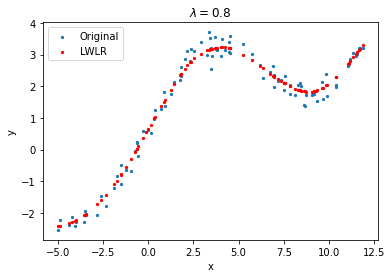
\includegraphics[width=0.5\textwidth]{2dii.png}
\end{figure}

\subsubsection*{iii}
\begin{figure}[htbp]
    \centering
    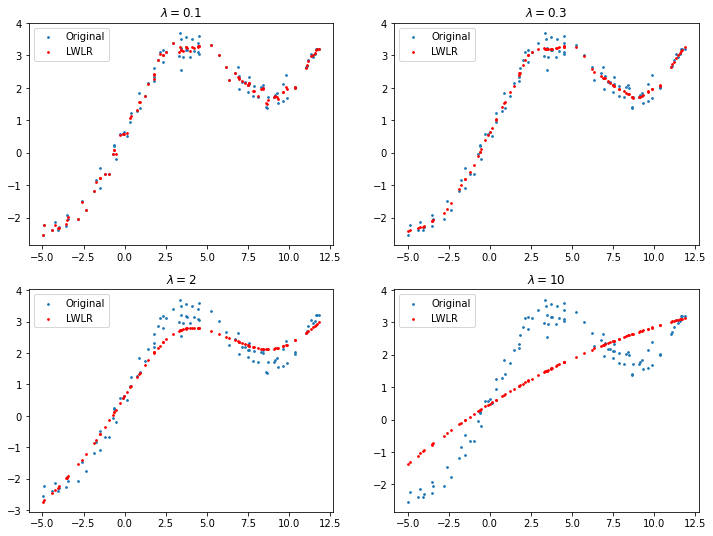
\includegraphics[width=0.6\textwidth]{2diii.png}
\end{figure}
When $\tau$ is too small, an over-fit occurs. When $\tau$ is too large, an under-fit occurs.

\newpage

\section{Derivation and Proof}

\subsection*{a}
Suppose we have $\widehat{Y_i} = \omega_0 + \omega_1 X_i$. To minimize the error 
$$E = \sum_{i=1}^{N}(Y - \widehat{Y_i})^2 = \sum_{i=1}^{N}(Y - \omega_0 - \omega_1 X_i)^2$$
we do partial differentiation for $\omega_0$ and $\omega_1$ respectively:
$$\frac{\partial E}{\partial \omega_0} = -2 \sum_{i=1}^{N}(Y_i - \omega_0 - \omega_1 X_i) = 0$$
$$\frac{\partial E}{\partial \omega_1} = -2 \sum_{i=1}^{N}(Y_i - \omega_0 - \omega_1 X_i) X_i = 0$$
Solving the first equation we can get
$$\sum_{i=1}^{N}Y_i - N\omega_0 - \omega_1\sum_{i=1}^{N}(X_i)$$
Thus,
$$\omega_0 = \frac{1}{N}(\sum_{i=1}^{N}Y_i - \omega_1 \sum_{i=1}^{N}X_i) = \bar{Y} - \omega_1 \bar{X}$$
Similarly, solving the second equation we can get
$$\sum_{i=1}^{N}X_i Y_i - \omega_0 \sum_{i=1}^{N}X_i - \omega_1 \sum_{i=1}^{N} X_i^2 = 0$$
Thus,
$$\omega_1 = \frac{\sum_{i=1}^{N}X_i Y_i - \bar{Y}\sum_{i=1}^{N}X_i}{\sum_{i=1}^{N}X_i^2 - \bar{X}\sum_{i=1}^{N}X_i}$$

\subsection*{b}
\subsubsection*{i}
Necessity: \\
According to the question, $\mathbf{A} = \mathbf{U} \mathbf{\Lambda} \mathbf{U}^T$, where $\mathbf{\Lambda} = diag(\lambda_1, \lambda_2, \cdots, \lambda_N)$, so we have for any $\mathbf{z} \neq 0$
$$\mathbf{z}^T \mathbf{A} \mathbf{z} = \mathbf{z}^T \mathbf{U} \Lambda \mathbf{U}^T \mathbf{z} = \mathbf{z^\prime} \mathbf{\Lambda} \mathbf{z^\prime}^T = \sum_{i=1}^{N} \lambda_i (z_{i}^{\prime})^2$$
Since $\lambda_i > 0$, we can prove $\mathbf{A}$ is PD. \\
Sufficiency: \\
As $\mathbf{A}$ is symmetric and PD, according to the concept of eigenvalue, we have $\mathbf{A}x = \lambda x$. We multiply $x^T$ on both sides and get
$$x^T\mathbf{AX} = \lambda x^T x = \lambda \sum_{i = 0}^{N} x_i^2 > 0$$
Therefore we prove for any $\lambda_i > 0$, $\mathbf{A}$ is PD.

\subsubsection*{ii}
Since $\mathbf{\Phi}^T\mathbf{\Phi}$ is symmetric, we can express it as $\mathbf{\Phi}^T\mathbf{\Phi} = \mathbf{U}\mathbf{\Lambda}\mathbf{U}^T$, where $\mathbf{\Lambda} = diag(\lambda_1, \lambda_2, \cdots, \lambda_N)$. So we have
$$\mathbf{\Phi}^T\mathbf{\Phi} + \beta\mathbf{I} = \mathbf{U}\mathbf{\Lambda}\mathbf{U}^T + \beta\mathbf{U}\mathbf{I}\mathbf{U}^T = \mathbf{U}(\mathbf{\Lambda}+\beta\mathbf{I}) \mathbf{U}^T$$
Therefore we prove the ridge regression has an effect of shifting all singular values by a constant $\beta$. \\
Let $\mathbf{\Lambda^{\prime}} = \mathbf{\Lambda} + \beta\mathbf{I}$, since $\beta > 0$, $\mathbf{\Lambda^{\prime}} = diag(\lambda_1^{\prime}, \lambda_2^{\prime}, \cdots, \lambda_N^{\prime})$ where $\lambda_i^{\prime} > 0$. So we have for any $\mathbf{z} \neq 0$
$$\mathbf{z}^T(\mathbf{\Phi}^T\mathbf{\Phi} + \beta\mathbf{I}) \mathbf{z} = \mathbf{z}^T \mathbf{U}\mathbf{\Lambda^{\prime}}\mathbf{U}^T \mathbf{z} = \lambda_i^\prime \sum_{i=1}^{N} z_i^2$$
where $\mathbf{z^\prime} = \mathbf{z}^T\mathbf{U}$. \\
Therefore we prove $\mathbf{\Phi}^T\mathbf{\Phi} + \beta\mathbf{I}$ is PD.
 
\end{document}